\section{提案するサーバテスト手法}

\subsection{要件の考察}

構成管理ツール独立性とOS・ディストリビューション汎用性をいかに満たすかを考察する.

特定の構成管理ツールからの独立性を満たせない理由は2つある.ひとつは構成管理ツールがもつOS・ディストリビューション汎用性を利用するために,テストの実装が特定の構成管理ツールに依存していることである.

もうひとつはテストスイートでのテスト用VM構築フェーズが,特定の構成管理ツールのみ対応していることである.

OS・ディストリビューション汎用性が満たせないのは,テストがシェルコマンドを直接記述する実装になっており,OS・ディストリビューションの違いをテストコードを書く者自らが意識しないといけないからである.

この考察から,提案するテスト手法に必要な要件は以下の通りとなる.

\begin{enumerate}
  \item テストの実装を特定の構成管理ツールに依存しない
  \item テストスイートではなくテストのみに特化する
  \item OS・ディストリビューションの違いを利用者に意識させない
\end{enumerate}

\subsection{要件を満たすための手法の提案}

考察した要件を満たすために,まずはOS・ディストリビューション毎にコマンドを分離し,統一的なAPIでコマンドを呼び出すことができる汎用コマンド実行フレームワークを定義する.このフレームワークではまず構成管理ツール固有の振る舞い(パッケージインストール等)を抽出する.そして振る舞いをテストするためのAPIを定義する.更にAPIから呼び出されるコマンドをOS・ディストリビューション毎に定義する.APIとコマンド群の間にはOS・ディストリビューションを判別して自動で適したコマンドを返すレイヤーを設ける.これにより運用業務で発生するコマンド群,特に確認作業に必要なコマンド群の体系化・抽象化を行う.

次に,テストコードの記述の抽象性を高め可読性を上げるために,宣言的な記法で汎用コマンド実行フレームワークを操作できる制御テストフレームワークを定義する.このフレームワークではまず記法の定義を行う.次に記法内の各命令と実際に呼び出す汎用コマンド実行フレームワークのAPIメソッドをひもづける.

汎用コマンド実行フレームワークと制御テストフレームワークの仕組みおよびその関係を\figref{fig:framework}に示す.

\begin{figure}[tb]
  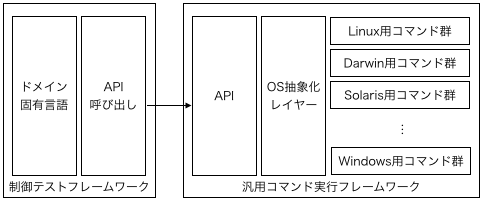
\includegraphics{framework-overview.png}
  \caption{汎用コマンド実行フレームワークと制御テストフレームワークの仕組みと関係}
  \label{fig:framework}
\end{figure}

\subsection{提案手法の実装}

提案手法に基づき実装した汎用コマンド実行フレームワークをspecinfra\cite{specinfra},制御テストフレームワークをserverspec\cite{serverspec}と名付けた.specinfra,serverspecともに実装にはRubyを採用している.Rubyを採用した理由はRSpecを利用するためである.RSpecはテストフレームワークとして実績があり,自然言語に近い形でテストコードを記述することができ,記法のカスタマイズが可能であることから採用した.

RSpecを採用することによりテストコードがどのように書けるのかをいくつかの例で示す.\figref{fig:test-files-with-serverspec}にserverspecによりファイルに対してテストを行うためのコードを示す.describeではテストの対象となるサーバ上のリソースを指定する.この図ではfile("/etc/passwd")などがそうである.これによりテスト対象が/etc/passwdというファイルであることを指定する.テストしたい内容はit \{ should ... \}といった形で記述する.例えば,it \{ should be\_file \}は,対象リソースがファイルとして存在する,ということを確認するためのコードである.

\begin{figure}[tb]
\setbox0\vbox{
\begin{verbatim}
describe file("/etc/password") do
  it { should be_file }
end

describe file("/tmp") do
  it { should be_directory }
end

describe file("/var/run/unicorn.sock") do
  it { should be_socket }
end

describe file("/etc/httpd/conf/httpd.conf") do
  its(:content) do
    should match /ServerName www.example.jp/
  end
end
\end{verbatim}
}
\centerline{\fbox{\box0}}
\caption{serverspecによりファイルをテストするためのコード\label{fig:test-files-with-serverspec}}
\end{figure}

\begin{figure}[tb]
\setbox0\vbox{
\begin{verbatim}
describe user("root") do
  it { should exist }
  it { should have_uid 0 }
  it { should belong_to_group "root" }
  it { should have_home_directory "/root" }
  it { should have_login_shell "/bin/bash" }
end
\end{verbatim}
}
\centerline{\fbox{\box0}}
\caption{serverspecによりシステムユーザに対するテストを実行するためのコード\label{fig:test-users-with-serverspec}}
\end{figure}

\begin{figure}[tb]
\setbox0\vbox{
\begin{verbatim}
describe group("root") do
  it { should exist }
  it { should have_gid 0 }
end
\end{verbatim}
}
\centerline{\fbox{\box0}}
\caption{serverspecによりシステムグループに対するテストを実行するためのコード\label{fig:test-groups-with-serverspec}}
\end{figure}

\begin{figure}[tb]
\setbox0\vbox{
\begin{verbatim}
describe package("httpd") do
  it { should be_installed }
end

describe package("serverspec") do
  it { should be_installed.by("gem") }
end

describe package("serverspec") do
  it do
    should be_installed.by("gem").with_version("0.14.3")
  end
end
\end{verbatim}
}
\centerline{\fbox{\box0}}
\caption{serverspecによりパッケージに対するテストを実行するためのコード\label{fig:test-packages-with-serverspec}}
\end{figure}

\begin{figure}[tb]
\setbox0\vbox{
\begin{verbatim}
describe service("ntpd") do
  it { should be_enabled }
  it { should be_running }
  it { should be_monitored_by("monit") }
end
\end{verbatim}
}
\centerline{\fbox{\box0}}
\caption{serverspecによりサービスに対するテストを実行するためのコード\label{fig:test-services-with-serverspec}}
\end{figure}

\begin{figure}[tb]
\setbox0\vbox{
\begin{verbatim}
describe port(80) do
  it { should be_listening }
end

describe port(80) do
  it { should be_listening.with("tcp") }
end

describe port(53) do
  it { should be_listening.with("udp") }
end
\end{verbatim}
}
\centerline{\fbox{\box0}}
\caption{serverspecによりポートに対するテストを実行するためのコード\label{fig:test-ports-with-serverspec}}
\end{figure}

\begin{figure}[tb]
\setbox0\vbox{
\begin{verbatim}
describe interface('eth0') do
  it { should have_ipv4_address("192.168.10.10") }
  its(:speed) { should eq 1000 }
end
\end{verbatim}
}
\centerline{\fbox{\box0}}
\caption{serverspecによりネットワークインターフェースに対するテストを実行するためのコード\label{fig:test-interfaces-with-serverspec}}
\end{figure}

\begin{figure}[tb]
\setbox0\vbox{
\begin{verbatim}
describe zfs('rpool') do
  it { should exist }
  it do
    should have_property {
      'mountpoint'  => '/rpool',
      'compression' => 'off'
    }
  end
end
\end{verbatim}
}
\centerline{\fbox{\box0}}
\caption{serverspecによりZFSに対するテストを実行するためのコード\label{fig:test-zfs-with-serverspec}}
\end{figure}

他に実装上重要な点として,テスト対象サーバに対して何もインストールする必要がないことが挙げられる.serverspecはインストールされたサーバに対してテストが実行できることはもちろん,インストールされていないサーバに対してもSSH経由でテストを実行することができる.また,提案手法に基づいて実装しているため,特定の構成管理管理ツールに依存せず,テストのみに特化し単機能である.単機能であるため他のツールとも組み合わせやすく,同種ツールとしてとりあげたTest Kitchenやrspec-systemには,ツール標準のテスト機構をserverspecで置き換えるbusser-serverspec\cite{busser-serverspec}やrspec-system-serverspec\cite{rspec-system-serverspec}が存在する.他にも,Vagrant\cite{vagrant}と連携してVMのテストを行うvagrant-serverspec\cite{vagrant-serverspec}というツールが存在する.
